\documentclass[runningheads,a4paper]{doc/llncs}
\usepackage[nolist,nohyperlinks]{acronym}
\usepackage{float, tabularx, array, booktabs}
\usepackage[T1]{fontenc}
\usepackage{mathpartir}
\usepackage{listings}
\usepackage{cleveref}
%\usepackage{amsmath}
%\usepackage{amsthm}
\usepackage{amssymb}
\usepackage{xcolor, colortbl}
\usepackage{soul}
\usepackage{wrapfig}

\definecolor{shyellow}{rgb}{.9, .8, .2}
\definecolor{shpurple}{rgb}{.9, .6, .8}

\newcommand{\hlmod}[1]{{%
    \sethlcolor{shyellow}\hl{#1}}%
}

\newcommand{\hlnew}[1]{{%
    \sethlcolor{shpurple}\hl{#1}}%
}


\acrodef{FOP}[FOP]{Feature Oriented Programming}
\acrodef{ITP}[ITP]{Interactive Theorem Prover}
\acrodef{FJ}[FJ]{Featherweight Java}
\acrodef{FFJ}[FFJ]{Feature Featherweight Java}
\acrodef{FFJ+}[FFJ\textsubscript{+}]{Overhaul Feature Featherweight Java}

\usepackage{amssymb}
\setcounter{tocdepth}{3}
\usepackage{graphicx}
\usepackage[misc]{ifsym}

\usepackage{hyperref}
\hypersetup{
    colorlinks=true,
    citecolor=blue,
    linkcolor=blue,
    filecolor=magenta,      
    urlcolor=cyan,
}

\usepackage{url}


\urldef{\mailsa}\path|abreu223@gmail.com|    
\newcommand{\keywords}[1]{\par\addvspace\baselineskip
\noindent\keywordname\enspace\ignorespaces#1}

\begin{document}

\mainmatter  % start of an individual contribution

% first the title is needed
\title{Mechanization and Overhaul of Feature Featherweight Java}

% a short form should be given in case it is too long for the running head
\titlerunning{Mechanization and Overhaul of Feature Featherweight Java}

% the name(s) of the author(s) follow(s) next
%
% NB: Chinese authors should write their first names(s) in front of
% their surnames. This ensures that the names appear correctly in
% the running heads and the author index.
%
\author{Pedro Abreu\textsuperscript{(\Letter)}%
%\thanks{Please note that the LNCS Editorial assumes that all authors have used
%the western naming convention, with given names preceding surnames. This determines
%the structure of the names in the running heads and the author index.}%
\and Rodrigo Bonif\'acio}
%
\authorrunning{Lecture Notes in Computer Science: Authors' Instructions}
% (feature abused for this document to repeat the title also on left hand pages)

% the affiliations are given next; don't give your e-mail address
% unless you accept that it will be published
\institute{Departamento de Ci\^encia da Computa\c{c}\~ao, Universidade de Bras\'{\i}lia, Brazil\\
\mailsa}
%
% NB: a more complex sample for affiliations and the mapping to the
% corresponding authors can be found in the file "llncs.dem"
% (search for the string "\mainmatter" where a contribution starts).
% "llncs.dem" accompanies the document class "llncs.cls".
%

\toctitle{Lecture Notes in Computer Science}
\tocauthor{Authors' Instructions}
\maketitle


\begin{abstract}
Specifying a language using an \ac{ITP} is seldom faithful
to its original pen-and-paper specification. However, the process of mechanizing a
language and type safety proofs might also unearth insights for improving the original 
specification. In this work, we detail %discuss
design decisions related to our process 
of first specifying \textit{\ac{FJ}} in \texttt{Coq} and then evolving 
such a specification to prove the type system properties of 
an overhaul version \textit{\ac{FFJ}}---a core-calculus for a family of %já é uma family of languages?
languages that address variability management in highly configurable systems, 
such as software product lines (SPLs); which we name as \textit{\ac{FFJ+}}. Indeed, \ac{FFJ+} 
is the first mechanization of \ac{FFJ}, and as such, it might also help researchers to 
derive proofs about software product line refinements without considering several 
assumptions about the underlining SPL assets. We believe 
that the whole process led us to a clearer, unambiguous, and equivalent syntax and semantics of 
\ac{FFJ}, while keeping the proofs, as well as our \ac{FJ} extensions, as simple as possible.

\keywords{Language Design, Language Semantics, Java, FOP, Coq}
\end{abstract}
 

\section{Introduction}
\textit{\acf{FOP}} \cite{prehofer_feature-oriented_1997} is a design methodology and tools for program synthesis \cite{batory_tutorial_2003}.
It aims at the modularization of software systems in terms of features. A \textit{feature}
implements a stakeholder's requirement and is typically an increment in program functionality.
When added to a software system, a feature introduce new structures, such as classes and methods,
and refines existing ones, such as extending methods bodies.

There are several \ac{FOP} languages and tools that provides varying mechanisms
that support the specification and composition of features properly, such as AHEAD \cite{batory_feature-oriented_2004},
FSTComposer \cite{apel_superimposition:_2008}, FeatureC++ \cite{apel_featurec++:_2005}, and more recently Delta-Oriented Programming \cite{schaefer_delta-oriented_2010}. \ac{FOP} has mostly been used to develop
\textit{product-lines} in disparate domains, including compilers for extensible Java dialects 
\cite{batory_jts:_1998}, fire support simulators for U.S. Army \cite{batory_achieving_2000}, high-performance network
\cite{batory_design_1992}, and program verification tools \cite{kurt_stirewalt_component-based_2001}.

Due to the relevance of \ac{FOP}, falar sobre lps...

Several attempts to formalize the type system of \ac{FOP} languages have been made. %Citar todas formalizações de delta oriented programmaning
For instance,  \textit{\acf{FFJ}} \cite{apel_feature_2008} is a proposed type system for \ac{FOP} languages and tools, 
which is developed on top of \textit{\acf{FJ}} \cite{igarashi_featherweight_2001}
to provide a simple syntax and semantics conforming with common \ac{FOP} languages, 
incorporating constructs for feature composition. %Falar de alguma formalizacao de DOP.

Nevertheless, none of the existing efforts for specifying \ac{FFJ} type system have been mechanized to date.
Which means that we have no formal guarantees that the specification is type-safe other than peer review. 
Such a method is known for enabling small errors to remain hidden for several years, specially as the proofs grow larger and harder to follow.
The idea behind mechanization is to check these proofs with the aid of a computer, reducing significantly the risk of errors, while 
taking full use of automation for the tedious or straightforward steps of the proof.

In this paper, we present an implementation of \ac{FJ} which we extend with \ac{FFJ} using \texttt{Coq}.
The process of scrutinizing \ac{FFJ} and defining \textit{unambigously} its semantics in \texttt{Coq} 
lead us to some language specification and implementation improvements. 
Henceforth, we refer this proposed calculus as \ac{FFJ+} to distinguish it when comparing our implementation to the original \ac{FFJ} design.
Altogether the improvements proposed in \ac{FFJ+} makes the transition more natural between \ac{FJ} and \ac{FFJ}, 
simplifying the auxiliary functions used in the language specification as well as the type safety proofs and lemmas. 
This allows defining \ac{FFJ+} with incremental changes to \ac{FJ} syntax and semantics, 
and consequently, incremental changes to proofs, leading to a clearer and simpler specification of \textit{FFJ}.
Hence we can summarize the main contribution of this paper as follows:
\begin{enumerate}
    \item The first mechanization of the \ac{FFJ} type system
    \item An improved specification of FFJ, which may help other researchers to reason about software product lines properties.
    \item A report about the benefits of using a proof assistant 
    to revamp an existing specification of a non-mechanized language type system.
\end{enumerate}

This paper is organized as follows: in the Section~\ref{seq:coq} we give a brief introduction to \texttt{Coq} 
Section~\ref{seq:fop} briefly introduces software product lines, \ac{FOP} and \ac{FFJ},
Section~\ref{seq:offj} gives a brief introduction of  \ac{FFJ+} and explains the main differences with \ac{FJ}
Section~\ref{seq:ffj} formally describes our revamped \ac{FFJ} and states the lemmas needed to preserve \ac{FJ} increment to \ac{FFJ} type safety, 
Section~\ref{seq:impl} discuss the implications of these results to the product line research,
Section~\ref{seq:related} discuss related works and
Section~\ref{seq:conclusion} is the conclusion and shows possible future works.


\section{Introduction to Coq}\label{seq:coq}
Lorem Ipsum

\section{Feature Oriented Programming}\label{seq:fop}

Feature-oriented programming (FOP) is a development approach 
that supports the \emph{stepwise refinement strategy} for software 
constructions~\cite{batory-tse2004}. Using FOP, a system is 
typically decomposed in (somewhat new) modular unities 
(named features) that resemble mixing layers~\cite{bracha-ecoop1990}, 
and thus are orthogonal to the typical object-oriented 
decomposition in terms of class hierarchies. 
Successful usage scenarios of FOP have been reported in the literature 
for the domains of highly configurable systems and
software product lines~\cite{}.  

\begin{wrapfigure}{r}{0.45\textwidth}
\centering
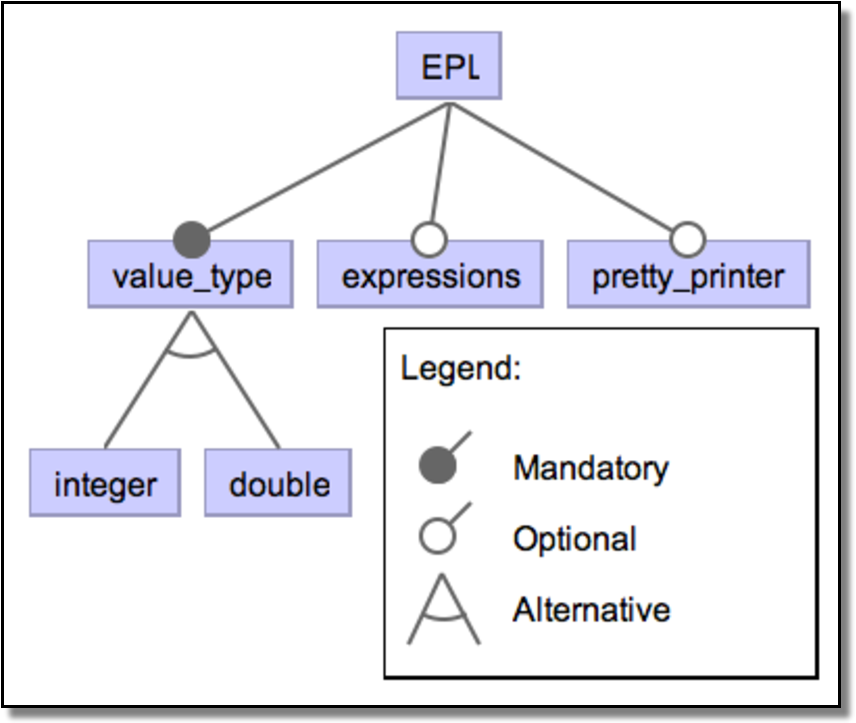
\includegraphics[scale=0.35]{doc/images/epl_fm}
\label{fig:epl_fm}
\caption{EPL feature model} 
\end{wrapfigure} 

FOP has been implemented using both programming 
language extensions and tooling support, such as 
Java AHEAD Tool Suite~\cite{batory_feature-oriented_2004} and \textsc{FeatureC++}~\cite{apel_featurec++:_2005}. 
In this section we illustrate the use of FOP through an AHEAD implementation 
of a slight adaptation of the Expression Product Line (EPL)~\cite{}---Figure~\ref{fig:epl_fm} shows 
the EPL feature model. Regarding our design decisions, 
in this case we implemented the mandatory features using a \textsc{base} AHEAD package (Figure~\ref{fig:epl-base}), which
declares a class hierarchy involving an interface (\texttt{Expression}) and
several classes (\texttt{Value}, \texttt{BinaryExpression}, \texttt{AddExpression}, and 
\texttt{SubExpression}), and one AHEAD package for each non-mandatory feature (see Figure~\ref{fig:epl-features}). Note 
that an AHEAD package contains eihter (a) plain Java entities (class or interface) declarations or (b) 
Java entities refinements. A refinement 
might refine methods declared in other packages or introduce new attributes or methods 
in existing classes or interfaces.  

\begin{figure}[htb]
\centering{
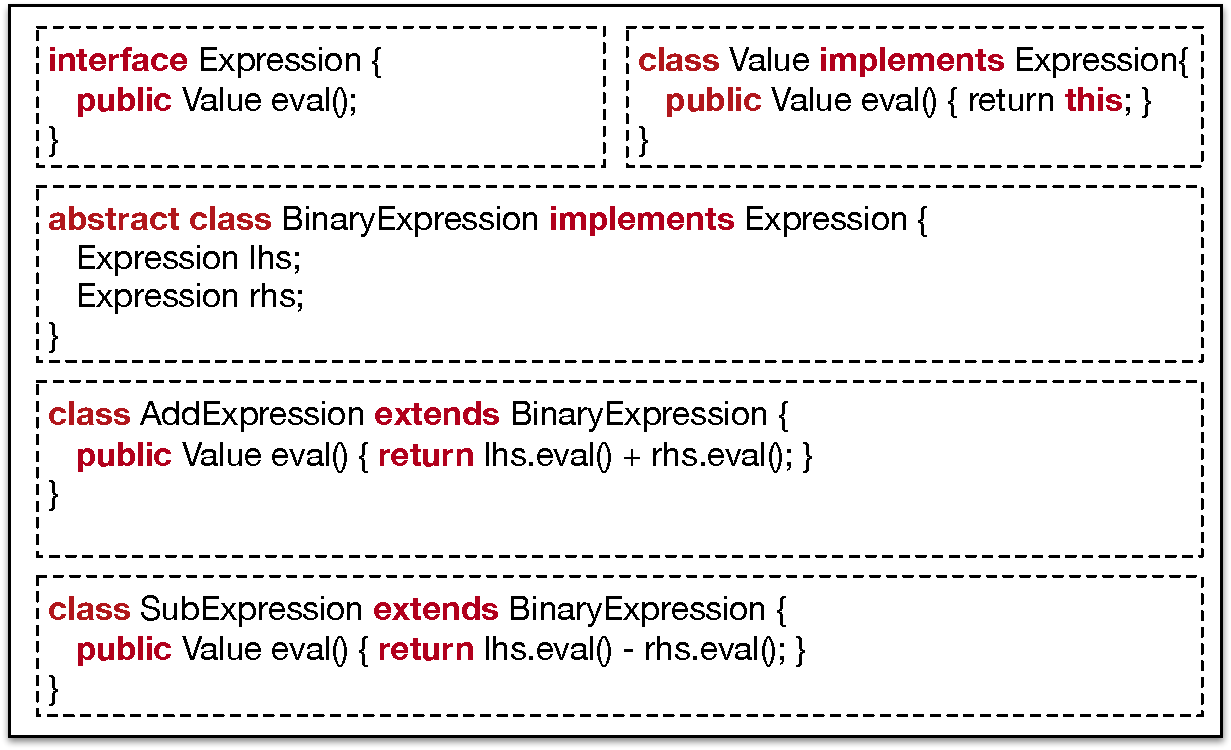
\includegraphics[scale=0.5]{doc/images/base.pdf}
}
\label{fig:epl-base}
\caption{The \textsc{base} package of the Expression Product Line}
\end{figure} 

The details of the EPL AHEAD non-mandatory feature packages are as follows. 

\begin{itemize}
\item Features \texttt{integer} and {double} refine the \texttt{Value} class of 
the \textsc{Base} package by introducing a new attribute named 
\texttt{value}, either with type \texttt{int} or \texttt{double}. According 
to the EPL feature model, only one of these features might be selected for 
a given product. 

\item The \texttt{expressions} feature introduces two new expressions 
to those declared in the \textsc{Base} package, one for multiplication 
and another for division. This particular feature does not refine 
existing classes, only introduces new ones. 

\item The \texttt{pretty\_printer} feature introduces the support for 
\emph{pretty printing} expressions. It refines the \texttt{Expression} 
interface and the \texttt{BinaryExpression} and \texttt{Value} classes, 
introducing a new method \texttt{print()} and also a 
new attribute (\texttt{operator}) for the \texttt{BinaryExpression} class.

\end{itemize}


\begin{figure}[htb]
\centering{
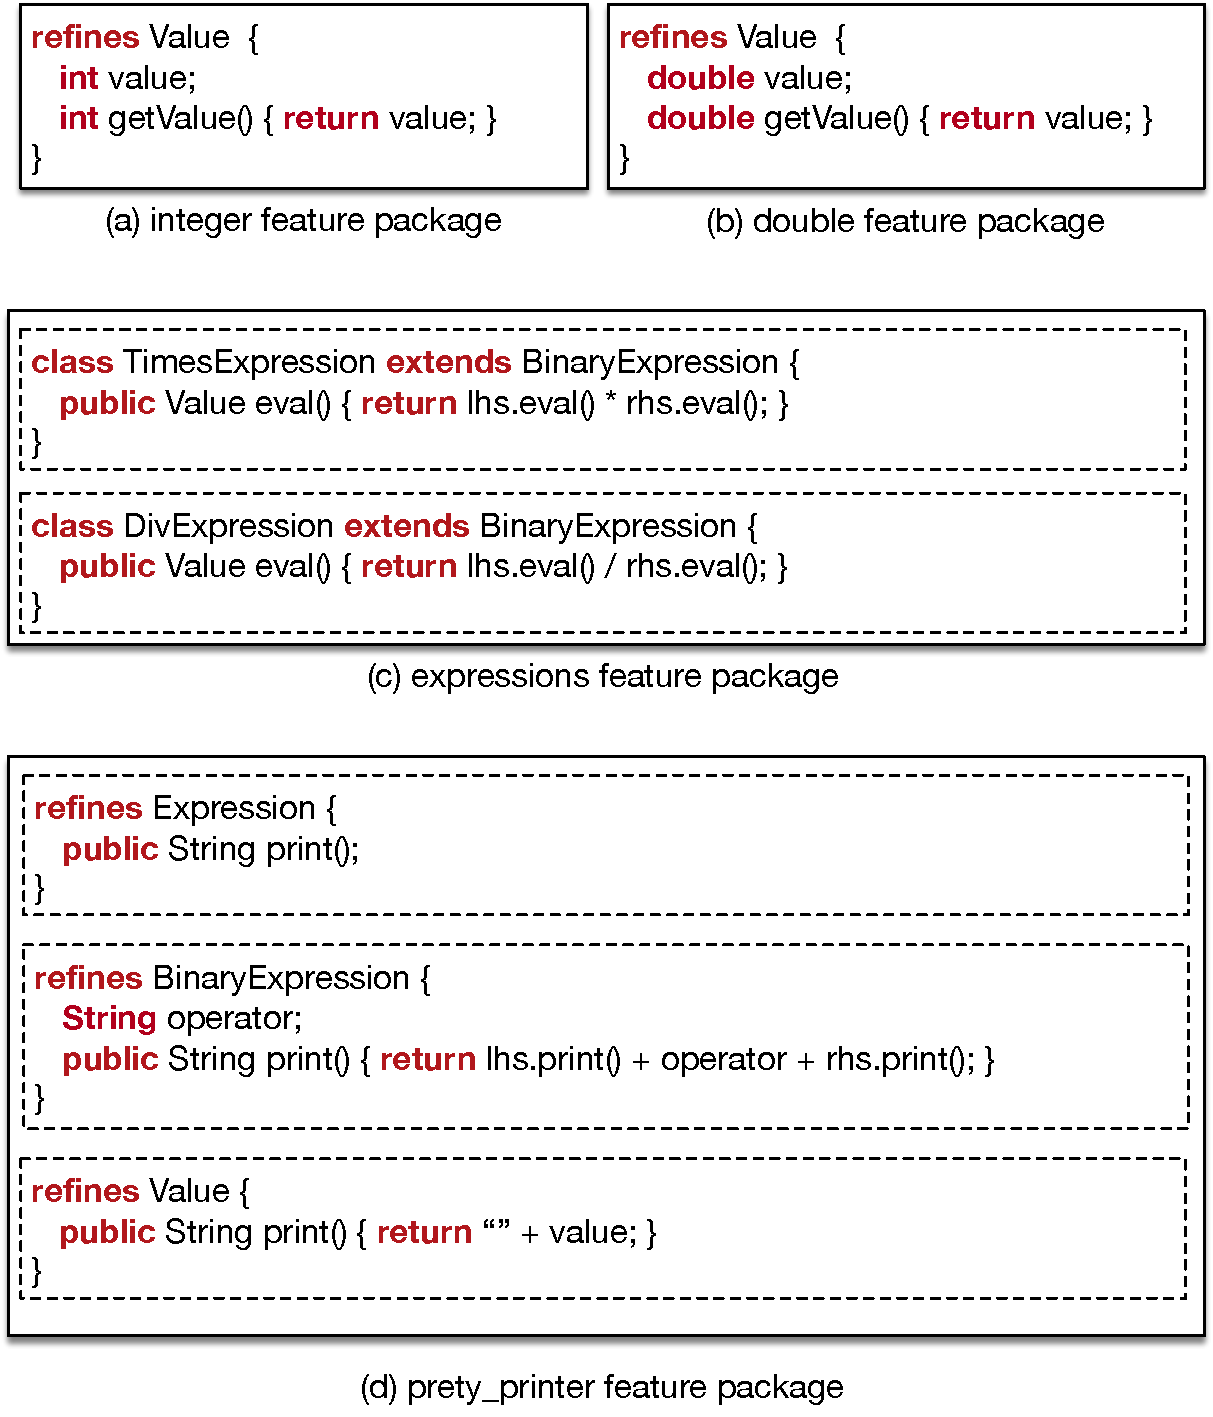
\includegraphics[scale=0.5]{doc/images/features.pdf}
}
\label{fig:epl-features}
\caption{Non-mandatory feature implementations of the Expression Product Line}
\end{figure} 

{\color{red}TODO: discutir o resultado de gerar um produto na EPL}

{\color{red}TODO: talvez combinar essa com a pr\'{o}xima se\c c\~{a}o.}


\subsection{Overview of \ac{FFJ} and \ac{FFJ+}}\label{seq:offj}

\acf{FFJ} is a core calculus for \acf{FOP}, which was built 
upon an extension of \acf{FJ}---a minimal subset of Java. 
In \ac{FFJ}, classes can be added and modified by the 
introduction of a new feature, that is, 
an existing class can be extended by a class refinement. 
A class refinement is declared like a conventional class, though 
preceded by the keyword \texttt{refines}. For example, 
\texttt{refines class C \{$\dots$\}} refers to a class
refinement that
\emph{refines} the class \texttt{C}. The same can be achieved 
for method introduction and modification. Methods refinement,
however, override a previous definition of the corresponding 
method.
 
% \ac{FJ} models a minimal subset of Java. \ac{FFJ} extends \ac{FJ} for \ac{FOP}.
To fully mechanize \ac{FFJ}, we had to disambiguate and enhance 
the language to some extent that it  deserves the attention of 
formally documenting these changes. 
Even though these changes are significant, as discussed in Section~\ref{seq:ffj}, 
the philosophy of \ac{FFJ}, \ac{FOP}, and Stepwise Refinement are maintained.
Due to the lack of space we will not provide neither the formal definition 
of \ac{FJ} nor \ac{FFJ}, but we refer the reader the original formalization of \ac{FJ}~\cite{igarashi_featherweight_2001}.
 and \ac{FFJ}~\cite{apel_feature_2008}
In \ac{FFJ}, as well as in \ac{FFJ+}, classes can be added and 
modified by the introduction of a new feature (as discussed in the previous section).
An existing class can be extended by a class refinement. A class refinement is declared like a class but
preceded by the keyword \texttt{refines}. For example, \texttt{refines class C@feat \{$\dots$\}} refers to a class refinement that
refines the class \texttt{C}. The same can be achieved for method introduction and modification. Methods refinement,
however, will override the previous definition.

A syntactical difference between \ac{FFJ} and \ac{FFJ+} is that, in \ac{FFJ+}, 
the feature notion appears in the abstract syntax tree (AST) of the language.
While the designers of \ac{FFJ} argue that the programmer does not have 
to explicitly state which feature a class or method belongs to, 
we favored the approach of stating the feature in the name of every refinement.
This greatly simplifies the structure of the formalism of the language and can be 
seen as an information gathered by the parser to build the AST, and thus 
the actual code expressed using the concrete syntax of this language 
might not have these annotations.

In addition, an \ac{FFJ+} program has a table with every class 
declaration (\textsf{CT}) and another table with every class refinement (\textsf{RT}).
We make this distinction to simplify the extension from \ac{FJ} in \texttt{Coq}, since 
with this decision we eliminate the need to match whether a class in the table 
is a refination or a declaration. From this \textsf{RT} we can retrieve the composition order
of the refinements and build the refinement chain of the program, 
which is used to check if features were composed correctly and
does not references features that have not been introduced yet. 
Notice that we redefine the denotation of \textsf{RT} from \ac{FFJ}.
In the original version, it was used to retrieve the refinement name given a 
refinement declaration. This is no longer necessary in \ac{FFJ+}, since
that information is already encoded in the syntax.

Finally, in the original definition of \ac{FFJ}, the lookup functions are 
somewhat circumvoluted. Accordingly, we propose a very different approach
for them, with the aim as been not only as formal and simple as possible, 
but also easy to evolve from our mechanized version of \ac{FJ}. 
To this end, we eliminate the need for reverse field lookup, reverse method lookup, 
and the refinement relation. A formal description with all these changes 
is given in Section~\ref{subsec:lookup}. Note that, we were only 
able to conceive these improvements while formalizing \ac{FFJ+} in 
\texttt{Coq}. 



\section{Overhaul Feature Featherweight Java}\label{seq:ffj}

\subsection{Syntax}
The Syntax of \ac{FFJ} is a straightfoward \ac{FOP} extension of \ac{FJ}. Due to the lack
of space we do not present the formal definition \ac{FJ} nor \ac{FFJ}, but instead we follow
the same scheme of the \ac{FFJ} original definition in \cite{apel_feature_2008} and present
the modified rules from \ac{FFJ} to \ac{FFJ+} highlighted with \hlmod{shaded yellow boxes} 
and new rules highlighted by \hlnew{shaded purple boxes}. Also notice that the sucessor and 
the refinement relations were simply dropped for being unecessary by now.

\newcommand{\cdecl}[6]{\texttt{class #1 extends #2 \{\={#3} \={#4}; #5 \={#6}\}}}
\newcommand{\crefine}[6]{\texttt{refines class #1 \{\={#2} \={#3}; #4 \={#5} \={#6}\}}}
\newcommand{\mdecl}[5]{\texttt{#1 #2 (\={#3} \={#4}) \{return #5;\}}}
\newcommand{\mrefine}[5]{\texttt{refines #1 #2 (\={#3} \={#4}) \{return #5;\}}}

\begin{table}[!ht]
    \begin{tabularx}{.62\textwidth}{l|}
        \hlnew{\texttt{R}~::=} \hfill \textit{refinement names:} \\
        \quad \hlnew{\texttt{C@feat}} \\ \\
        \texttt{CD}~::= \hfill \textit{class declarations:}\\
        \quad \cdecl{C}{D}{C}{f}{K}{M} \\  \\
        \hlmod{\texttt{CR}~::=} \hfill \textit{class refinements:}\\
        \quad \hlmod{\texttt{refines class R \{\={C} \={f}; KD \={M} \={MR}\}}} \\ \\
        \texttt{K}~::=  \hfill\textit{constructor declarations:}\\
        \quad \texttt{C(\={C}~\={f})\{super(\={f});~this.\={f}=\={f};\}}\\\\
        \texttt{KD}~::= \hfill\textit{constructor refinements:} \\
        \quad \texttt{refines~C(\={E}~\={h}, \={C} \={f})\{original(\={f}); this.\={f}=\={f};\}} \\\\
        \texttt{M}~::= \hfill\textit{method declarations:}\\
        \quad \mdecl{C}{m}{C}{x}{e}
    \end{tabularx}
    \begin{tabularx}{.4\textwidth}{l}
        \texttt{MR}~::= \hfill \textit{method refinements:}\\
        \quad \mrefine{C}{m}{R}{x}{e} \\ \\
        \texttt{e}~::= \hfill \textit{expressions:}\\
        \quad \texttt{x} \hfill\textit{variable}\\ 
        \quad \texttt{e.f} \hfill\textit{field access}\\
        \quad \texttt{e.m(\={e})} \hfill\textit{method invocation}\\
        \quad \texttt{new~C(\={e})} \hfill\textit{object creation}\\
        \quad \texttt{(C)e} \hfill\textit{cast}\\ \\
        \texttt{v}~::= \hfill \textit{values:}\\
        \quad \texttt{new~C(\={e})} \hfill\textit{object creation}
    \end{tabularx}
    \quad
    \caption{\ac{FFJ} Syntax}
    \label{abstractsyntax}
\end{table}
%\end{center}


The syntax of \ac{FFJ+} constructs is given at Table~\ref{abstractsyntax}. The metavariables
\texttt{A}, \texttt{B}, \texttt{C}, \texttt{D} and \texttt{E} ranges over class names, \texttt{f} and \texttt{g} range over
field names; \texttt{m} ranges method name; \texttt{x} ranges over variable, \texttt{v} ranges over
values, \texttt{feat} ranges over feature names. We assume that the set of variables includes the special variable \texttt{this}, which
cannot be used as the name of an argument of a method.

We write \texttt{\=f} as a shorthand for a possible empty sequence \texttt{f\textsubscript1}, \dots, \texttt{f\textsubscript{n}} 
and similarly for \texttt{\=C}, \texttt{\=x}, \texttt{\=e}, etc. We abbreviate the operations on pairs of sequences
``\texttt{\=C~\=f}'' for ``\texttt{C\textsubscript1~f\textsubscript1},\dots, \texttt{C\textsubscript{n}~f\textsubscript{n}}''
and ``\texttt{this.\=f=\=f;}'' as a shorthand for 
``\texttt{this.\=f\textsubscript1=\=f\textsubscript1;} \dots, \texttt{this.\=f\textsubscript{n}=\=f\textsubscript{n};}''.
We write empty sequence as $\bullet$.


A class declaration \texttt{class\ C~extends~D\ \{\={C} \={f}; K \={M}\}} 
introduces a class \texttt{C} with superclass \texttt{D}. This class has fields \texttt{\=f}
of type \texttt{\=C}, a constructor \texttt{K} and methods \texttt{\=M}. The fields of the class \texttt{C}
is \texttt{\=f} added to the fields of its superclass \texttt{D}, all of them must have distinct names.
Methods, on the other hand, may override another superclass method with the same name.
Method override in both \ac{FFJ} and \ac{FFJ+} is basically method rewriting. 
Methods are uniquely identified by its name, i.e. overloading is not supported.

A class refinement \texttt{refines~class~C@feat~\{\={C}~\={f};~KD~\={M}~\={MR}\}}
introduces a refinement of the class \texttt{C} and belongs to the feature \texttt{feat}. 
This refinement contains the fields  \texttt{\=f} of type \texttt{\=C}, 
a constructor refinement \texttt{KR}, methods declarations \texttt{\=M} and method refinements $\overline{\texttt{MR}}$.
Like class declarations, the fields of a class refinement \texttt{R} are added to the fields of its predecessor, which
is explained in more detail in Section \ref{subsec:lookup}.

Constructor declaration \texttt{C(\={C}~\={f})\{super(\={f}); this.\={f}=\={f};\}} and a constructor refinement 
\texttt{refines~C(\={E}~\={h}, \={C}~\={f}) \{original(\={f}); this.\={f}=\={f};\}} introduce a constructor 
for the class \texttt{C} with fields \texttt{\=f} of type \texttt{\=C}. The constructor declaration body is simply 
a list of assignment of the arguments with its correspondent field preceded by calling its superclass constructor with the correspondent arguments.
The constructor refinement only differs from constructor declaration that instead of calling the superclass constructor
it will call its predecessor constructor (denoted by \texttt{original}).

Method declaration \texttt{C~m~(\={C}~\={x})\ \{return~e;\}} and method refinement \texttt{refines C~m~(\={C}~\={x})\ \{return~e;\}} 
introduce a method \texttt{m} of return type \texttt{C} with arguments \texttt{\={C}~\={x}} and body \texttt{e}.
Method declarations can only appear inside a class declarations or refinement, whereas method refinement should only appear
inside a class refinement. There is such a distinction between method declaration and method refinement for allowing the type checker
to recognize the difference between method refinement and inadvertent overriding/replacement.

A class table \textsf{CT} is a mapping from class names \texttt{C} to class declarations \texttt{CD}.
A refinement table \textsf{RT} is a mapping from refinement name \texttt{C@feat} to refinement declarations.
An \ac{FFJ} program consists of a triple (\textsf{CT}, \textsf{RT}, \texttt{e}) of a class table, a refinement table
and an expression. Throughout the rest of the paper the \textsf{CT} and the RT are assumed to be always fixed to lighten the notation.

\subsection{Lookup Functions}\label{subsec:lookup}

In \ac{FFJ} as well as in \ac{FJ} types are classes and classes have a subclass relation defined by the syntax of class declaration.
To navigate this subclass relation in the \textsf{CT}, the auxiliary operator \texttt{<:} is given in Table \ref{table:sub_pred}, this operator is 
the reflexive and transitive closure of the subclass relation.

The \textsf{CT} is expected to satisfy some sanity conditions:
\begin{itemize}
	\item  \textsf{CT}~(\texttt{C}) = \texttt{class C}$\ldots$ for every \texttt{C} $\in$ dom(\textsf{CT})
	\item \texttt{Object} $\notin$ dom(\textsf{CT})
	\item for every class name \texttt{C}~(except \texttt{Object}) appearing anywhere
		in \textsf{CT}, we have \texttt{C} $\in$ dom(\textsf{CT})
	\item there are no cycles in the subtype relation induced by \textsf{CT}, i.e., the
		relation \texttt{<:} is antisymmetric
\end{itemize}

\begin{table}[!ht]

    \raggedright \textit{Subtyping}\\
	\centering
	\begin{tabular}{c@{\qquad}c@{\qquad}c}
		\inferrule{ }{\texttt{C~<:~C}} & 
		\inferrule{\texttt{C <: D} \qquad \texttt{C <: E}}
		{\texttt{C~<:~E}} &
		\inferrule{\texttt{class~C~extends~D~\{~\ldots~\}}}
		{\texttt{C~<:~D}} \\
	\end{tabular}
    \vspace*{2pt}
    \caption{Subtype Relation}
    \label{table:sub_pred}
\end{table}


In \ac{FFJ+} we fetch the refinement precedence via its position in the \textsf{RT}, i.e.
if a refinement of a class appears first in the \textsf{RT} it will be applied first. 
These functions to navigate the \textsf{RT} are all defined in Table \ref{table:refinement}
    
First we have the function $class\_name$ which retrieves the name of a class refinement.

Next we define the function $refinements\_of~\texttt{C}$ to retrieve the refinements of 
a given class in the same order as they were introduced in the \textsf{RT}.

To navigate the precedence we define the \textit{pred} and the \textit{last} functions.
The \textit{pred} function will get a class refinement as an argument,
filter refinements of the same class of \texttt{R} as \texttt{\=R}, fetch the $index$ $n$ of \texttt{R} in \texttt{\=R} 
and return the element \texttt{P} at the position $n-1$ in \texttt{\=R} (denoted by the $get$ function). Notice that \textit{pred} is a partial function
because it is not defined if the a refinement is the first refinement.

The \textit{last} function retrieves the last refinement of a given class \texttt{C}.
This is needed because in \ac{FFJ+} we navigate the refinement chain backwards, from the last refinement
to the first, looking for a given method or field. 

\begin{table}[!ht]
	\def\arraystretch{2.5}
    \raggedright \hlnew{\textit{Class Name}}\\
	\centering
    \begin{tabular}{c}
        \rowcolor{shpurple}
        \inferrule{ \texttt{R} = \texttt{C@feat}}
                    {class\_name~\texttt{R} = \texttt{C} }
    \end{tabular}

    \qquad\qquad \\ 
    \raggedright \hlnew{\textit{Refinements of a class}}\\
	\centering
    \begin{tabular}{c}
        \rowcolor{shpurple}
        \inferrule{ filter~(\lambda R \cdot class\_name~\texttt{R} == \texttt{C})~\textsf{RT} = \texttt{\=R}}
                    {refinements\_of~\texttt{C} = \texttt{\=R} }
    \end{tabular}

    \raggedright \hlmod{\textit{Predecessor}}\\
	\centering
    \begin{tabular}{c}
        \rowcolor{shyellow}
        \inferrule{refinements\_of~(class\_name~\texttt{R}) = \texttt{\=R}\\
                  index~\texttt{R}~\texttt{\=R}~=~n\\
                  get~(n-1)~\texttt{\=R}~=~\texttt{P}}
        {\textit{pred}~\texttt{R}~=\texttt{P}}
    \end{tabular}

    \raggedright \hlmod{\textit{Last}}\\
	\centering
    \begin{tabular}{c}
        \rowcolor{shyellow}
        \inferrule{refinements\_of~\texttt{C} = \texttt{\=R}\\
                  tail~\texttt{\=R}~=~\texttt{R}}
        {\textit{last}~\texttt{C}~=\texttt{R}}
    \end{tabular}

    \qquad\qquad
    \caption{Refinement Relations}
    \label{table:refinement}
\end{table}

With this in hand we can define the actual lookup functions $fields$, $mtypes$ and $mbody$.
They are taken directly from \ac{FFJ} definition, with a new hypothesis and an extra rule.
The extra rule and hypothesis makes reference to dealing with the refinements. This is necessary
to make the proofs easier to maintain, since all we need to do is to provide a few acceptance lemmas
about these new lookup functions which we name $fields_R$, $mtype_R$ and $mbody_R$.

$fields_R$ simply retrieves the fields of all refinements up to that point in the refinement chain.

$mtype_R$ and $mbody_R$ tries to find the last introduction to a method, and retrieves its type or body.
Notice that these two definitions greatly differs from \ac{FFJ} to \ac{FFJ+}. In \ac{FFJ} $mtype$ would
retrieve the typing of the first method introduction, whereas in \ac{FFJ+} it will retrieve the
type of the last method refinement, and only later we define the rules for guarantying that the
refinement always has the same type of the method declaration. This was made to greatly simplify
the proof that states that if a method has $mtype$ then it also has a $mbody$, since both 
functions follows the same structure the proof is straightforward.


\begin{table}[ht!]
	\centering
	\begin{tabular}{c}
        \rowcolor{shpurple}
        \inferrule{\texttt{refines R \{\=C \=f; KR \=M \={MR}\}} \qquad
                    \neg pred~\texttt{R}}
                {fields_R~\texttt{R}~=~\texttt{\=C \=f}} \\
        \\
        \rowcolor{shpurple}
		\inferrule{\texttt{refines R \{\=C \=f; KR \=M \={MR}\}} \qquad
                    \textit{pred}~\texttt{R}~=~\texttt{P}}
                {fields_R~\texttt{C}=fields_R~\texttt{P, \={C} \={f}}}\\
        \\
	\end{tabular}
	\centering
	\begin{tabular}{c}
		$fields~$\texttt{Object}$=\bullet$ \\
        \\
        \rowcolor{shyellow}
		\inferrule{\texttt{class C extends D \{\=C \=f; K \=M\}} \qquad 
                    \neg\textit{last}~\texttt{C}}
                {fields~\texttt{C}=fields~\texttt{D, \={C} \={f}}} \\
        \\
        \rowcolor{shyellow}
		\inferrule{\texttt{class C extends D \{\=C \=f; K \=M\}} \qquad 
                    \textit{last}~\texttt{C}~=~\texttt{R}}
                {fields~\texttt{C}=fields~\texttt{D, \={C} \={f},} fields_R~\texttt{R}}\\
        \\
	\end{tabular}
    \label{table:field}
    \caption{Field lookup}
\end{table}

\newcommand{\mtype}[2]{\ensuremath{mtype~(\texttt{#1},\texttt{#2})}}
\newcommand{\mtyper}[2]{\ensuremath{mtype_R~(\texttt{#1},\texttt{#2})}}
\newcommand{\mrettype}[2]{\texttt{\={#1}}\ensuremath{~\rightarrow~}\texttt{#2}}

\begin{table}[h!]
	\centering
	\begin{tabular}{c}
        \rowcolor{shpurple}
        \inferrule{\crefine{R}{C}{f}{KR}{M}{MR} \qquad 
                \mdecl{B}{m}{B}{x}{e} \in \texttt{\={M}}}
                {\mtyper{m}{R}~=~\mrettype{B}{B}} \\ 
    \end{tabular}
    \vspace*{.2cm}
    \begin{tabularx}{.55\textwidth}{c}
        \rowcolor{shpurple}
        \inferrule{\crefine{R}{C}{f}{KR}{M}{MR} \qquad 
                \texttt{m} \notin \texttt{\={M}} \\
                \mrefine{B}{m}{B}{x}{e} \in \overline{\texttt{MR}}}
                {\mtyper{m}{R}~=~\mrettype{B}{B}} \\ 
    \end{tabularx}
    \begin{tabularx}{.39\textwidth}{c}
        \rowcolor{shpurple}
        \inferrule{\crefine{R}{C}{f}{KR}{M}{MR} \\\\
                \texttt{m} \notin \texttt{\={M}} \quad
                \texttt{m} \notin \overline{\texttt{MR}} \quad
                pred~\texttt{R}~=~\texttt{P}}
                {\mtyper{m}{R}~=~\mtyper{m}{P}} \\ 
    \end{tabularx}
    \vspace*{2pt}
    \begin{tabular}{c}
        \rowcolor{shyellow}
        \inferrule{\cdecl{C}{D}{C}{f}{K}{M} \qquad 
                \mdecl{B}{m}{B}{x}{e} \in \texttt{\={M}} \\
                last~\texttt{C}~=~\texttt{R} \qquad
                \neg\mtyper{m}{R}}
                {\mtype{m}{C}~=~\mrettype{B}{B}} \\ 
        \\
        \rowcolor{shyellow}
        \inferrule{\cdecl{C}{D}{C}{f}{K}{M} \qquad 
                    \texttt{m}\notin~\texttt{\={M}} \\\\
                    last~\texttt{C}~=~\texttt{R} \qquad
                    \neg\mtyper{m}{R}}
		{\mtype{m}{C}~=~\mtype{m}{D}} \\
        \\
        \rowcolor{shyellow}
        \inferrule{\cdecl{C}{D}{C}{f}{K}{M} \qquad 
                    last~\texttt{C}~=~\texttt{R}} 
		{\mtype{m}{C}~=~\mtyper{m}{R}} \\

	\end{tabular}
    \quad\\
    \label{mtypelookup}
    \vspace*{5pt}
    \caption{Method type lookup}
\end{table}

\newcommand{\mbody}[2]{\ensuremath{mbody~(\texttt{#1},\texttt{#2})}}
\newcommand{\mbodyr}[2]{\ensuremath{mbody_R~(\texttt{#1},\texttt{#2})}}
\newcommand{\mretbody}[2]{\texttt{\={#1}}\ensuremath{.}\texttt{#2}}

\begin{table}[h!]
	\centering
	\begin{tabular}{c}
        \rowcolor{shpurple}
        \inferrule{\crefine{R}{C}{f}{KR}{M}{MR} \qquad 
                \mdecl{B}{m}{B}{x}{e} \in \texttt{\={M}}}
                {\mbodyr{m}{R}~=~\mretbody{x}{e}} \\ 
    \end{tabular}
    \vspace*{.2cm}
    \begin{tabularx}{.55\textwidth}{c}
        \rowcolor{shpurple}
        \inferrule{\crefine{R}{C}{f}{KR}{M}{MR} \qquad 
                \texttt{m} \notin \texttt{\={M}} \\
                \mrefine{B}{m}{B}{x}{e} \in \overline{\texttt{MR}}}
                {\mbodyr{m}{R}~=~\mretbody{x}{e}} \\ 
    \end{tabularx}
    \begin{tabularx}{.39\textwidth}{c}
        \rowcolor{shpurple}
        \inferrule{\crefine{R}{C}{f}{KR}{M}{MR} \\\\
                \texttt{m} \notin \texttt{\={M}} \quad
                \texttt{m} \notin \overline{\texttt{MR}} \quad
                pred~\texttt{R}~=~\texttt{P}}
                {\mbodyr{m}{R}~=~\mbodyr{m}{P}} \\ 
    \end{tabularx}
    \vspace*{2pt}
    \begin{tabular}{c}
        \rowcolor{shyellow}
        \inferrule{\cdecl{C}{D}{C}{f}{K}{M} \qquad 
                \mdecl{B}{m}{B}{x}{e} \in \texttt{\={M}} \\
                last~\texttt{C}~=~\texttt{R} \qquad
                \neg\mbodyr{m}{R}}
                {\mbody{m}{C}~=~\mretbody{x}{e}} \\ 
        \\
        \rowcolor{shyellow}
        \inferrule{\cdecl{C}{D}{C}{f}{K}{M} \qquad 
                    \texttt{m}\notin~\texttt{\={M}} \\\\
                    last~\texttt{C}~=~\texttt{R} \qquad
                    \neg\mbodyr{m}{R}}
		{\mbody{m}{C}~=~\mbody{m}{D}} \\
        \\
        \rowcolor{shyellow}
        \inferrule{\cdecl{C}{D}{C}{f}{K}{M} \qquad 
                    last~\texttt{C}~=~\texttt{R}} 
		{\mbody{m}{C}~=~\mbodyr{m}{R}} \\

	\end{tabular}
    \quad\\
    \label{mbodylookup}
    \vspace*{5pt}
    \caption{Method Body lookup}
\end{table}

Override function in~\ref{table:override} inductively guaranties that a method refinement respects the 
type a method was introduced for the first time, which can be in a super class or in a previous
refinement.

\begin{table}
	\centering
	\begin{tabular}{c}
    	\inferrule{\mtype{m}{D}~=~\mrettype{D}{D}~implies~\overline{\texttt{C}}~=~\overline{\texttt{D}}~and~\texttt{C}_0~=~\texttt{D}}
       			  {override~\texttt{m D \=C C}_0}
    \end{tabular}
    \begin{tabular}{c}
    	\\\rowcolor{shpurple}
    	\inferrule{\cdecl{C}{D}{C}{f}{K}{M}\qquad
        			\mdecl{C$_0$}{m}{C}{x}{e} \in \texttt{\=M}\\\\
                    \neg~pred~\texttt{R}\qquad \texttt{R}~=~\texttt{C@feat}\qquad
                    }
        		  {override_R~\texttt{m R \=C C}_0}\\
        \\\rowcolor{shpurple}
        \inferrule{\crefine{P}{C}{f}{KR}{M}{MR}\qquad
        			\mdecl{C$_0$}{m}{C}{x}{e} \in \texttt{\=M}\\\\
                    pred~\texttt{R}~=~\texttt{P}\qquad
                    }
        		  {override_R~\texttt{m R \=C C}_0}\\
        \\\rowcolor{shpurple}
        \inferrule{\crefine{P}{C}{f}{KR}{M}{MR}\qquad
        			\texttt{m}\notin\texttt{\=M}\\\\
                    pred~\texttt{R}~=~\texttt{P}\qquad
                    override_R~\texttt{m P \=C C}_0
                    }
        		  {override_R~\texttt{m R \=C C}_0}
    \end{tabular}
    \vspace*{2pt}
    \caption{Override Function}
    \label{table:override}
\end{table}

Introduce in~\ref{table:introduce} function checks if a method was not yet declared earlier in the refinement chain.
\begin{table}
	\centering
	\begin{tabular}{c}
    	\rowcolor{shpurple}
    	\inferrule{pred~\texttt{R}~=~\texttt{S}\qquad
        			\neg~\mtyper{m}{S}}
                    {introduce~\texttt{m R}}\\ \\
    	\rowcolor{shpurple}
        \inferrule{\neg~pred~\texttt{R}\qquad 
                    \texttt{R}~=~\texttt{C@feat} \qquad
                    \cdecl{C}{D}{C}{f}{K}{M}\qquad
        			\texttt{m} \notin \texttt{\=M}}
                    {introduce~\texttt{m R}}
    \end{tabular}
    \vspace*{2pt}
    \caption{Introduce Function}
    \label{table:introduce}
\end{table}

\begin{table}[h!]
    \centering
    \begin{tabular}{c}
    	\rowcolor{shpurple}
        \inferrule{\mathtt{\bar{x}: \bar{C}, this: C~\vdash t_0 : E_0\qquad E_0 <: C_0 } \\ \\
            \mathtt{CT(C)~=class~C~extends~D~\{\dots\}\qquad
            \mathnormal{override}(m, D, \bar{C}\rightarrow C)}}
            {\mathtt{C_0~m~(\bar{C}~\bar{x})\{return~t_0;\}~OK~in~C}}\\\\

    	\rowcolor{shpurple}
        \inferrule{\mathtt{\bar{x}: \bar{C}, this: C~\vdash t_0 : E_0\qquad E_0 <: C_0 \qquad R~=~C@feat} \\ \\
                \mathtt{CT(C)~=class~C~extends~D~\{\dots\}\qquad RT(R)~=~refines~R~\{\dots~\bar{M}~\dots\}}\\ \\
                \mathtt{\mathnormal{override}(m, D, \bar{C}\rightarrow C) \qquad \mathnormal{introduce}~m~R\qquad m \in \bar{M}}}
            {\mathtt{C_0~m~(\bar{C}~\bar{x})\{return~t_0;\}~OK~in~R}}\\\\

        \rowcolor{shpurple}
        \inferrule{\mathtt{\bar{x}: \bar{C}, this: C~\vdash t_0 : E_0\qquad E_0 <: C_0 \qquad R~=~C@feat} \\ \\
                \mathtt{RT(R)~=~refines~R~\{\dots~\bar{M},~\overline{MR}~\dots\} \qquad m\notin\bar{M} \qquad m\in\overline{MR}}\\ \\
                \mathtt{\mathnormal{override_R}(m, R, \bar{C}\rightarrow C) \qquad \mathnormal{introduce}~m~R}}
            {\mathtt{refines~C_0~m~(\bar{C}~\bar{x})\{return~t_0;\}~OK~in~R}}\\\\

    \end{tabular}
\label{typing2}
\caption{Method typing in \ac{FFJ+}}
\end{table}

\begin{table}[h!]
    \centering
    \begin{tabular}{c}
    	\rowcolor{shpurple}
        \inferrule{\mathtt{K~=~C~(\bar{D}~\bar{g},~\bar{C}~\bar{f})~\{super(\bar{g});~this.\bar{f}=\bar{f}\}\qquad
            \mathnormal{fields}(D)~=~\bar{D}~\bar{g} \qquad \overline{M}~OK~in~C}}
            {\mathtt{\cdecl{C}{D}{C}{f}{K}{M}~OK}}\\\\

    	\rowcolor{shpurple}
        \inferrule{\mathtt{ \overline{M}~OK~in~R\qquad \overline{MR}~OK~in~R}}
            {\mathtt{\crefine{R}{C}{f}{KR}{M}{MR}~OK}}\\\\
    \end{tabular}
\label{typing2}
\caption{Class and refinement typing in \ac{FFJ+}}
\label{table:classtyping}
\end{table}

Every class and refinement of a \ac{FFJ+} program is assumed to respect the well-formednes rules
defined in~\ref{table:classtyping}.

\subsection{Typing and Reduction}
The typing and computation rules for expressions are elided since are the same as \ac{FJ}. An environment
$\Gamma$ is a finite mapping from variables to types, written $\bar{c}:\bar{C}$.
The typing judgment for expressions has the form $\Gamma \vdash e: C$, read ``in
the environment $\Gamma$, expression $e$ has type $C$''.

The reduction relation is of the form $e \rightarrow e'$, read ``expression
$e$ reduces to expression $e'$ in one step'', We write $\rightarrow *$ for the
reflexive and transitive closure of $\rightarrow$.

There are three reduction rules, one for field access, one for method invocation, and one for casting.
We write $[\bar{d}=\bar{x}, e=y]e_0$ for
the result of replacing $x_1$ by $d_1$, $x_2$ by $d_2, \dots, x_n$ by $d_n$, and $y$ by $e$ in
the expression $e_0$.

Notice that with the absence of side effects, there is no need of stack
or heap for variable binding. 




\section{Implications}\label{seq:impl}

\section{Related Work}\label{seq:related}

\section{Conclusion}\label{seq:conclusion}


\bibliography{doc/bibliography}{}
\bibliographystyle{doc/splncs03}



%\begin{thebibliography}{5}
%\end{thebibliography}

%esta parte fica para outra sesssao
%The main idea of \ac{FFJ} is to provide a timeline of increment to \ac{FJ} classes and methods called refinements. With that in hand, job of
%proving that \ac{FFJ} maintain \ac{FJ} type safety comes down to showing that the refinements respects former typing rules. And that job is 
%fairly easy given that \ac{FFJ} syntax does not affect \ac{FJ} typing rules.

\end{document}
